\chapter{Quantitative analysis of Lightning network privacy}

\label{Chapter07LNattacks}

We evaluate the possibility of various attacks on Lightning, considering various subsets of nodes potentially compromised.

Payment channels suffer from security vulnerabilities, such as the wormhole attack~\cite{Malavolta2019}, anonymity issues~\cite{Malavolta2017}, and scalability limitations related to  the upper bound on the number of concurrent payments per channel~\cite{EmelyanenkoK2017}, which have been pointed out by the scientific community but never quantitatively analyzed. 

In this work, we first analyze the proneness of the LN to the wormhole attack and attacks against anonymity. 
We observe that an adversary needs to control only $2\%$ of LN nodes to learn sensitive payment information (e.g., sender, receiver and payment amount) or to carry out the wormhole attack. 
Second, we study the management of concurrent payments in the LN and quantify its negative effect on scalability. 
We observe that for micropayments, the forwarding capability of up to $50\%$ of channels is restricted to 
a value smaller than the overall channel capacity.
This phenomenon not only hinders scalability but also opens the door for DoS attacks: We estimate that 
a network-wide DoS attack costs within $1.5M$~USD, while isolating the biggest community from the rest of the network costs only $225k$~USD.

Our findings should prompt the LN community to consider the security, privacy and scalability issues of the network studied in this work 
when educating users about path selection algorithms, as well as to adopt multi-hop payment protocols that provide stronger security, privacy and 
scalability guarantees. 

We perform a quantitative analysis of LN's resistance to three previously described attacks on privacy.
\footnote{Our research is concerned with the definition of the LN as described in the BOLTs and thus the results apply equally to every implementation.}

Privacy in payment networks is defined in terms of value privacy (the attacker does not know how much is sent) and relationship anonymity (the attacker does not know who is paying whom).
In the LN, an additional definition is added: a wormhole attack allows an adversary to steal fees from honest intermediaries and temporarily block their funds.
How much of a threat do these attacks present?
This depends on a multiple factors: for an attack to be successful, a payment must pass through a path partially controlled by the attacker.
For the three attacks, we estimate this probability based on a simulated network for an array of parameters.
Our findings suggest that LN, as of 2019, depends on highly connected and highly capitalized nodes: in case a relatively small proportion of such nodes are compromised, the attacker succeeds with a high probability.


\section{Datasets}
\label{sec:datasets}



We obtained a snapshot of LN on 2020-02-25 from \url{https://ln.bigsun.xyz} and parsed with the (anonymized) scripts available at~\cite{Tikhomirov2019}.
%\footnote{Our experiments are based on data from \url{https://ln.bigsun.xyz/}.
%	The (anonymized) scripts are available at~\cite{LightningPrivacy}.}
This snapshot consists of $5929$~nodes and $35233$~channels.
We model this data as an undirected multi-graph (i.e., may contain multiple edges between each pair of nodes), 
representing the fact that several channels can be shared by two LN nodes.
We only considered the largest connected component, 
which contains $5862$~nodes $(98.87\%)$ and $35196$~channels $(99.89\%)$.
We observe that this subgraph contains a representative sample of the LN.
We refer to this dataset as \emph{LN20}.

Based on \emph{LN20}, 
LN nodes have an average degree of $12.01$ and a median degree of $3$ (see~\cref{fig:node-degree-histogram,fig:channel-capacity-histogram}).
The majority of nodes have very few channels, 
whereas there is a small number of nodes with many channels. 
In particular, there are more than 1744 nodes with degree 1, and the most connected node has 1198~channels.
The capacity is also unequally distributed.
 %\footnote{Public key \texttt{03ffdd7fd4656a55a63a4b6e154325859681718ba2fac40e51cb61752506bb8c7b}.}
These observations motivate the methodology in our experiments in~\cref{sec:sec-priv-attacks}. 

We also derive a series of historic snapshots which represent the state of LN on the first day of each month from April~2018 to February~2020.
We refer to this dataset as \textit{LNHist} 
and use it in the subsequent chapter, where we study of concurrent payments on LN performance over time.
\todo[inline]{Ref to future chapter doesn't work}
% (\ref{Chapter08HTLClimit}).
%See Appendix~\ref{sec:historic} for our study of the temporal evolution of the LN based on LNHist.


\begin{figure}[tb]
	\centering
	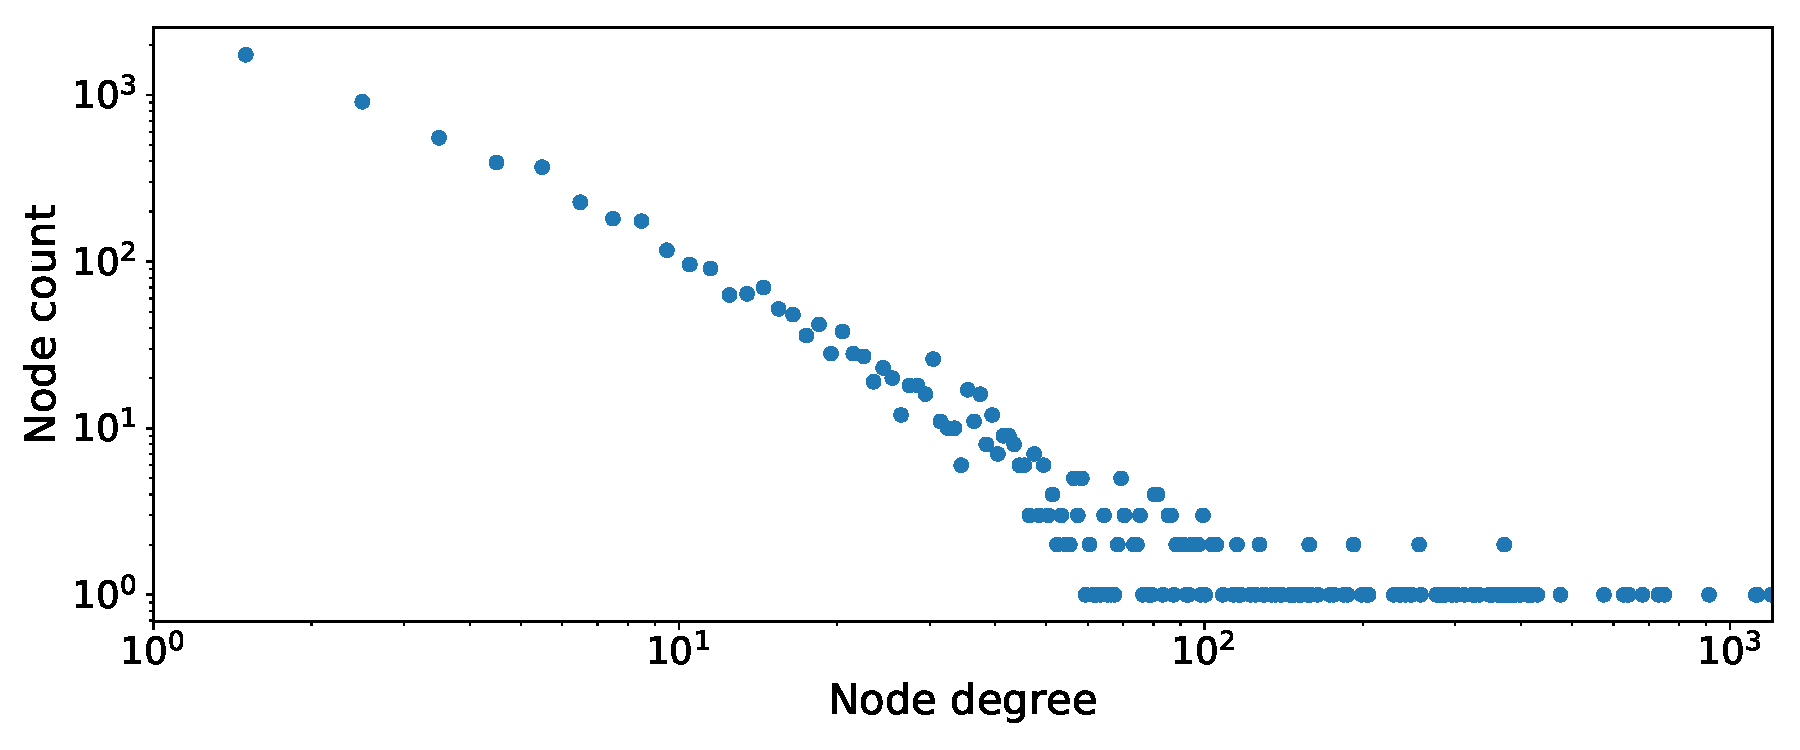
\includegraphics[width=\columnwidth]{node-degree-histogram}
	\caption{Node degree distribution.\label{fig:node-degree-histogram}}
\end{figure}

\begin{figure}[tb]
	\centering
	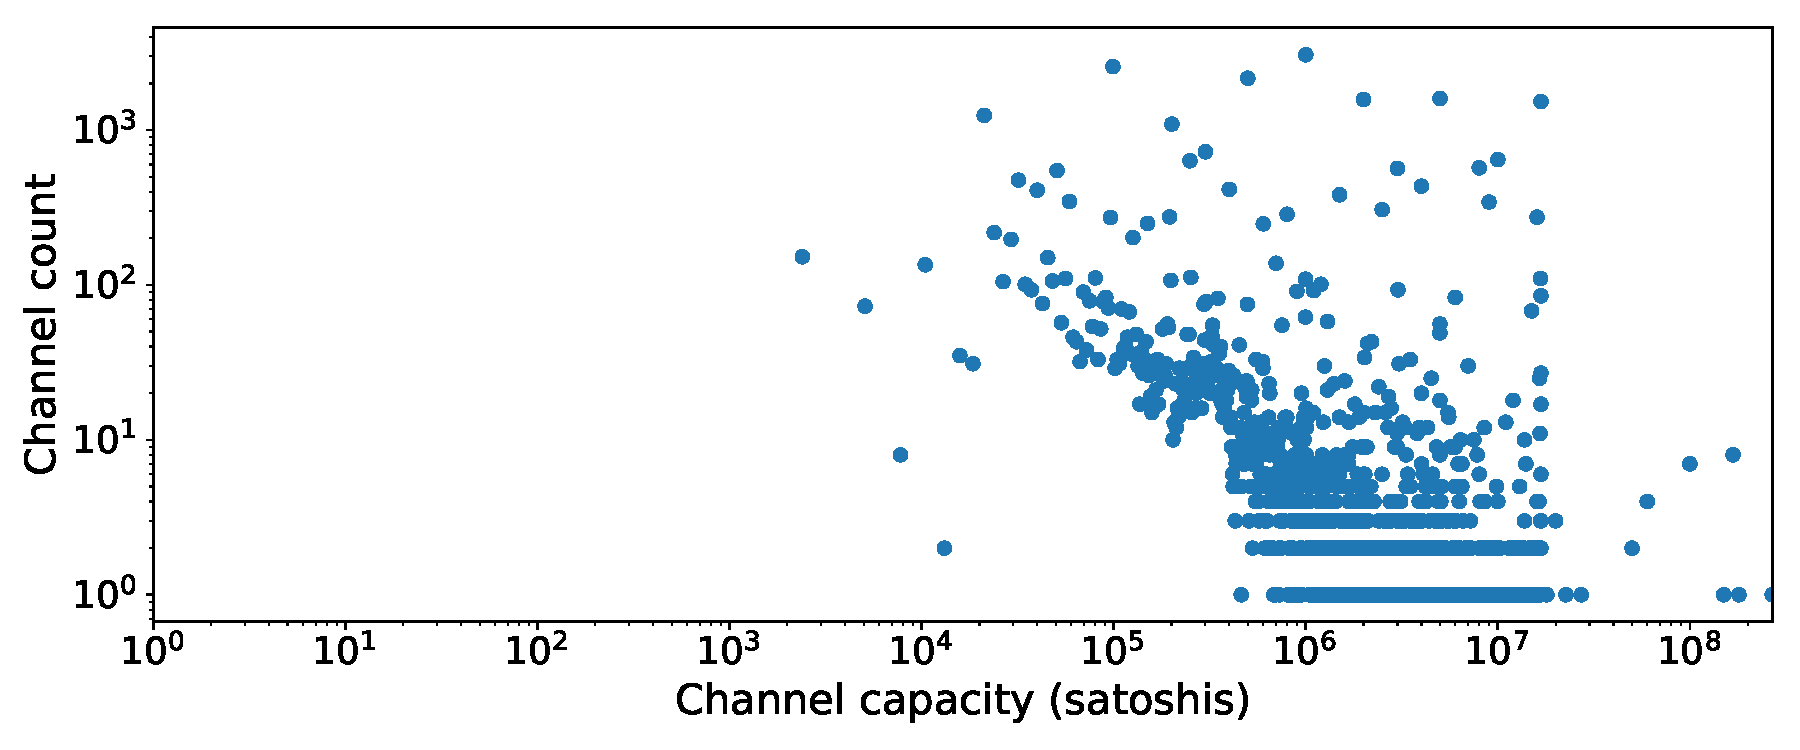
\includegraphics[width=\columnwidth]{channel-capacity-histogram}
	\caption{Channel capacity distribution.\label{fig:channel-capacity-histogram}}
\end{figure}

\subsubsection*{Ethical considerations} 
Our analysis is based solely on publicly available data. 
We do not interfere with the LN activity, nor deanonymize any of its nodes. 


\section{Security and privacy: theory and practice}
\label{sec:sec-priv-attacks}

As introduced in~\cref{sec:background}, the LN builds upon Hash Time-Lock Contracts aiming to achieve 
atomicity in multi-hop payments.
However,~\cite{Malavolta2019} argues that due to the \emph{wormhole attack} atomicity does not hold in LN.
Another LN study~\cite{Malavolta2017} shows that privacy of LN users and their transactions can be breached.
While the aforementioned works demonstrate the feasibility of these attacks, 
their effectiveness in practice depends, among other factors, on the topology of the LN.
In this experiment, we aim to identify the impact of these security and privacy issues in our snapshot of the LN.
%We study the prevalence of three attacks: the wormhole attack, value privacy, and relationship anonymity.
%We first describe our methodology, and then present the results for the three attacks along with the necessary background.

\subsection{Security and privacy attacks: background}

\begin{figure*}[tb]
	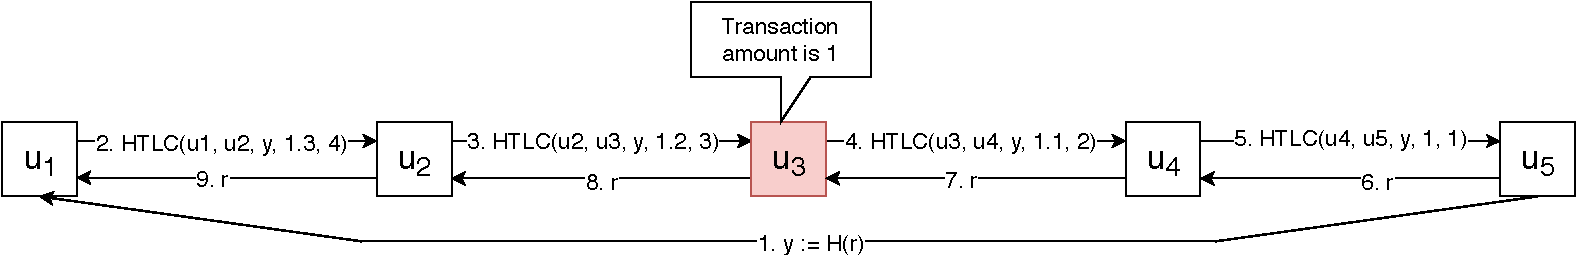
\includegraphics[width=\textwidth]{vp-figure.pdf}
	
	\vspace{0.3cm}
	
	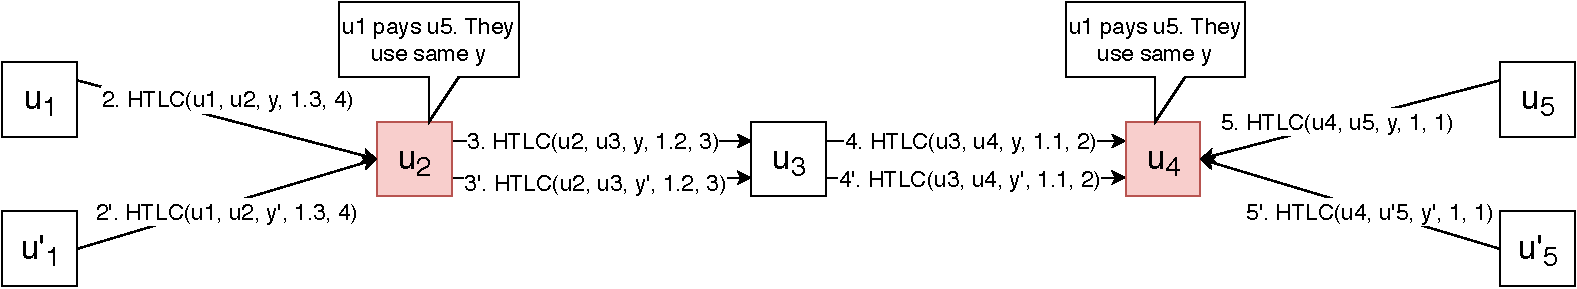
\includegraphics[width=\textwidth]{ra-figure.pdf}
	
	\vspace{0.3cm}
	
	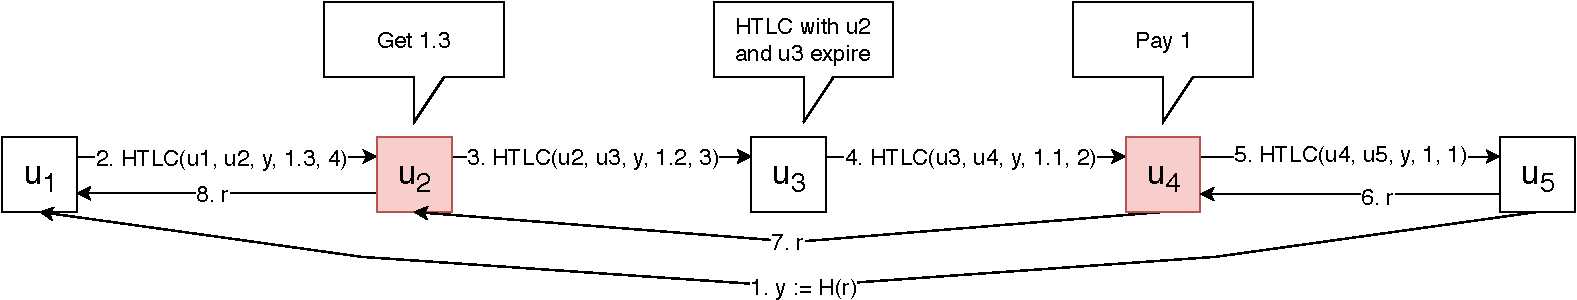
\includegraphics[width=\textwidth]{wa-figure.pdf}
	
	\caption{\label{fig:wormhole-attack} An illustrative example of value privacy (top), relationship anonymity (middle), and the wormhole attack (bottom).}
\end{figure*}

\subsubsection{Value privacy~\cite{Malavolta2017}}
Intuitively, value privacy ensures that for a transaction involving only honest users, 
corrupted users outside of the path learn no information about the transaction value.
This notion thus heavily relies on the existence of paths without adversarial nodes.  
Otherwise, an adversarial intermediary node can trivially learn the (upper bound of the) amount of a transaction that it forwards. 
For instance, in~\cref{fig:wormhole-attack} the adversary $u_3$
forwards $1.2$ coins to $u_4$, estimating the transaction amount at around $1$ coin plus forwarding fees.

\subsubsection{Relationship anonymity~\cite{Malavolta2017}}
Intuitively, relationship anonymity ensures that given two simultaneous transactions 
between two pairs of nodes $(u_1, u_2)$ and $(u'_1, u'_2)$ routed through the same path of intermediary 
users $i_1, \ldots, i_n$, the adversary controlling some of those intermediaries cannot tell who is paying to whom with probability better than $1/2$.
However, this is not achieved in the LN.
An adversary controlling $i_1$ and $i_n$ can use the cryptographic challenge included in the HTLC to 
determine who pays to whom.
For instance, in~\cref{fig:wormhole-attack} the adversary controlling $u_2$ 
and $u_4$ can determine that $u_1$ is transacting with $u_5$ as the same value $y$ is used along the whole path. 
Similarly, $u_2$ and $u_4$ can determine that $u'_1$ is transacting with $u'_5$ as the same $y'$ is being used along the path. 

\subsubsection{The wormhole attack~\cite{Malavolta2019}}
In the wormhole attack, two colluding nodes in a transaction path prevent honest intermediaries from 
participating in the successful completion of the payment, stealing the 
fees initially intended for honest intermediaries.\footnote{One may argue that this is not an attack, as from the sender's point of view the payment is delivered. Yet, this attack takes the economic incentive that honest users have to forward payments in the first place.} 
%On top of that, coins are locked in the HTLCs with honest 
%intermediaries longer than required for a successful transaction, thereby preventing honest users from 
%participating in other (possibly successful) transactions. 
An example of the wormhole attack is depicted in~\cref{fig:wormhole-attack}. 
Here, $u_4$ does not send the opening value $r$ to $u_3$ (step 7 in~\cref{fig:htlc}) to fulfill the HTLC previously set in this channel. 
Instead, $u_4$ sends the value $r$ to $u_2$ outside of the LN protocol, which allows $u_2$ to settle the HTLC with $u_1$. 
As a consequence, contracts with $u_3$ expire, simulating transaction failure and
preventing $u_3$ from participating in the successful completion of the transaction. 



\subsection{Methodology}
In this section, we describe how we study the proneness of the LN to attacks with respect to the value privacy, relationship anonymity, and wormhole attack scenarios. 

We first compute the paths between pairs of nodes.
Given a pair of nodes $u_1$ and $u_2$, 
we compute the list of paths that connect them with one restriction:
we consider only the paths with at most three intermediary nodes.
We observe that paths of this length suffice to allow more than $85\%$ of 
transactions between a random pair of nodes (\cref{fig:payment-success}).
% for transactions amounts expected in the LN \missing{add citation here}.
%We restrict our experiment to paths of this length because of high computational requirements 
%caused by significantly higher number of paths for higher length limit.
%Due to high computational requirements, we run a smaller number of randomized experiments for the higher path length limit.
%We remark that in the Lightning Network shorter paths are more likely to be chosen due to lower fees and higher probability of payment success.
We also note that these paths allow us to exemplify all attacks that we want to study in this experiment.
\begin{figure}
	\centering
	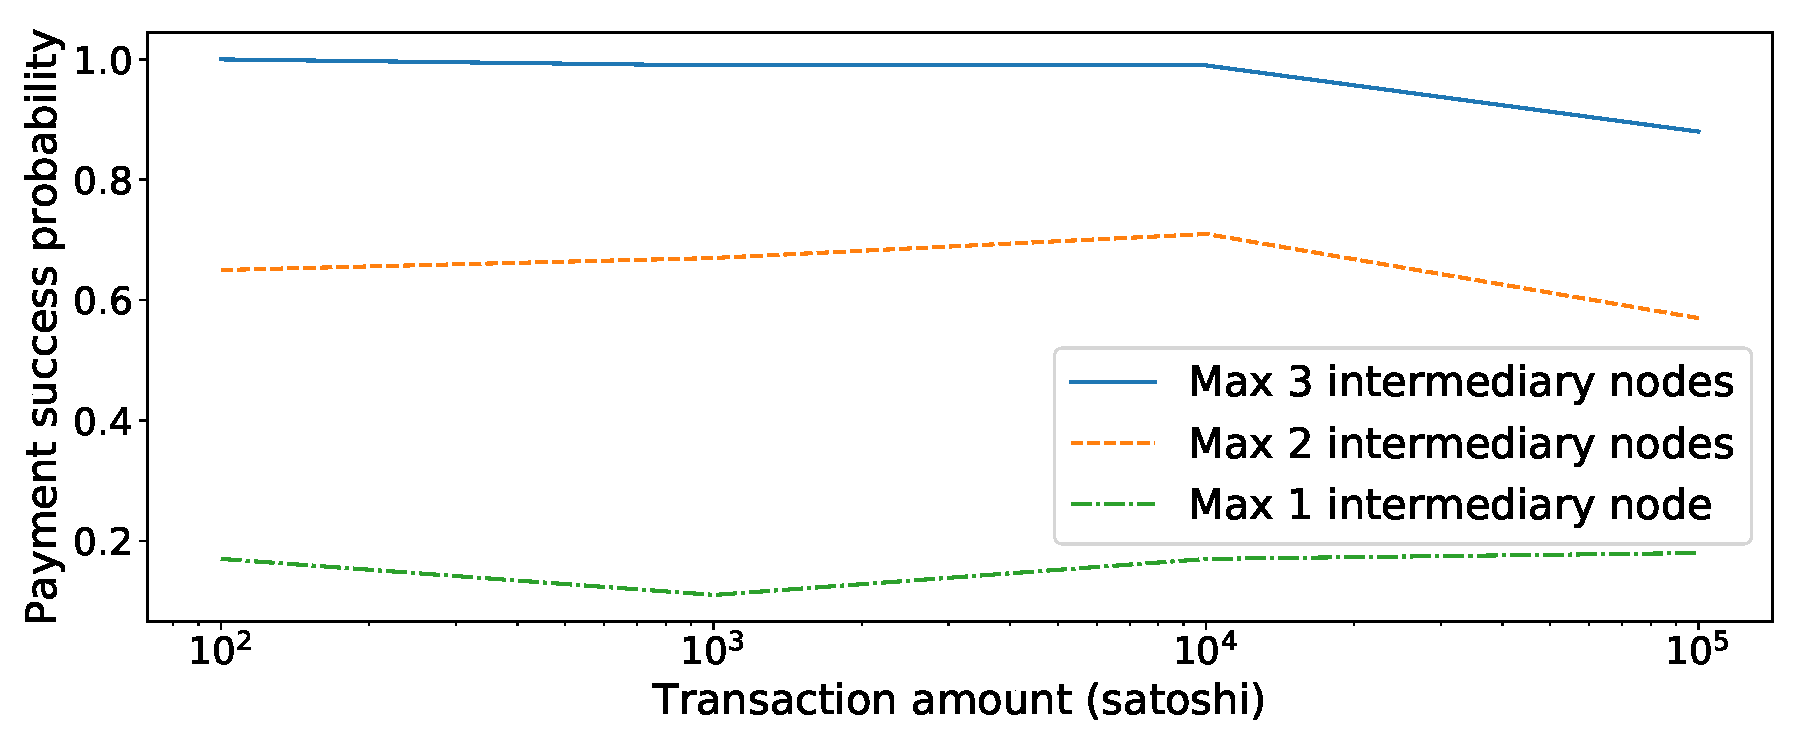
\includegraphics[width=\columnwidth]{payment-success}
	\caption{The share of experiment runs where paths with sufficient capacity exist between sender and receiver.}
	\label{fig:payment-success}
\end{figure}

%We also note that while LN protocol limits the length of paths at 20~hops, LN clients don't have to find all paths of lengths lower than the limit.
%Instead, they iterate through possible paths until the payment succeeds.

%We check the effectiveness of the wormhole attack by randomly selecting a representative sample of the population 
%of LN nodes composed of 1000~pairs of nodes.
%We set a payment amount $x$ for the experiment to one of the values: $10^2$, $10^3$, $10^4$, $10^5$ satoshis.
%For each pair of nodes ($u_1, u_2$), we obtain all possible paths connecting them that contain at most 
%five nodes (i.e., $u_1$, $u_2$ and up to three intermediary nodes).
%We restrict our experiment to paths of this length because of high computational requirements caused by significantly higher number of paths for higher length limit.
%The average number of paths between two random nodes is 24 with up to 4 nodes is 24, 3550~with up to 5 nodes, and approximately 200~thousand for up to 6 nodes.
%We limit our experiments to paths with at most 5~nodes, as this allows us to exemplify all attacks including the wormhole attack.
%Moreover, in the majority of cases the nodes would have paths shorter than 5~nodes (see below), and in the real network shorter paths are more likely to be chosen due to lower fees and lower chances of payment failure.
%Approx time for one experiment with 1000 iterations: 3 hops: tens of minutes, 4: ~4 hours, 5: ~days.

%We only consider $u_1$ with have a channel with the capacity not less than $x$.
%The rationale behind this restriction is the following.
%We aim to estimate the probability that a payment will traverse through a vulnerable path.
%When calculating routes, the sender only takes into account only the local channels with sufficient capacity.
%If there are no such channels, the payment is impossible regardless of the network structure.

Let $\textit{paths}_{\langle u_1, u_2 \rangle}$ be the set of paths between $u_1$ and $u_2$ thereby computed. 
We further prune the set $\textit{paths}_{\langle u_1, u_2 \rangle}$ into a subset 
$\textit{paths}_{\langle u_1, u_2 \rangle, x}$, containing  only the paths that 
allow to transfer at least $x$ satoshis. 
For instance, $\textit{paths}_{\langle u_1, u_2 \rangle, 10}$ 
contains the paths between $u_1$ and $u_2$ allowing to transfer at least $10$ satoshis. 


For a channel to be capable of transferring $x$ satoshis from $u_i$ to $u_j$, $u_i$ must have a balance of 
at least $x$ satoshis. However, the current balance of each counterparty in a channel is not publicly available. 
Thus, we consider a path suitable for a given transaction if the total capacity of every channel 
in the path is not lower than the transaction amount, independently of how this capacity 
is distributed among the two channel counterparties. 
This heuristic might consider a path suitable for a transaction while it is not.
We nevertheless follow this heuristic as it is also used by LN nodes in practice. 
%, which leads to payments trying multiple paths before succeeding.
% \missing{add reason why it is still ok to consider this heuristic - do we have other choice?}

%We estimate the share of cases when at least one suitable path exists for various values of $x$.
% results-1571154370.json (with has_path function)
%We arrive at the following shares of payments with at least one suitable path: 99.3, 99.2, 99.0, and 86.6 percent for 100, 1k, 10k, and 100k satoshis, respectively.
%The results indicate that while it is possible to find a path for smaller payments in the majority of cases, the Lightning network can not yet reliably support larger payments.\footnote{100k satoshis are equivalent to 100~USD at 10k USD per bitcoin.}
%The most likely explanation of the drop in success rate is the lack of incoming capacity at the receiver's side (see Section~\ref{sec:liquidity} for the measurement of liquidity -- a related metric).

%For each attack, we present the definition of a path prone to this attack.
%We consider all other paths safe.

As the next step, we study the effectiveness of the selected attack.
For a chosen transaction amount $x$,
we split the set $\textit{paths}_{\langle u_1, u_2 \rangle, x}$ into two subsets:
(i) $\textit{paths-prone}_{\langle u_1, u_2 \rangle, x}$: The subset of paths that are prone to the attack;
(ii) $\textit{paths-safe}_{\langle u_1, u_2 \rangle, x}$:  The subset of paths that are not susceptible to being attacked. 
The definition of a path of the form $u_1 \rightarrow i_1 \rightarrow  \ldots \rightarrow i_n \rightarrow u_2$  being 
prone to the attack depends on the type of the attack:
\begin{itemize}
	
	\item \textit{Value privacy:} We say that a path is prone to the 
	value privacy attack if any of the intermediary nodes is under adversarial control. 
	
	\item \textit{Relationship anonymity:} We say that a path  
	is prone to the relationship anonymity attack if nodes $i_1$ and $i_n$ are under adversarial control.
	
	\item \textit{Wormhole attack:} We say that a path  
	is prone to the wormhole attack if there exist two non-neighboring intermediary 
	nodes $i_j$ and $i_k$ that are under adversarial control (i.e., $j < k$ and $k \neq j + 1$). 
	
\end{itemize}

%We remark that there exist two differences in the definitions of a prone path in the wormhole attack and the relationship anonymity attack. 
%First, for the relationship anonymity attack we do not require that there is an honest user between the two adversarial nodes.
%For instance, a path of the form $u_1 \rightarrow i_1 \rightarrow i_2 \rightarrow u_2$ where $i_1$ and $i_2$ are under adversarial control,  would be considered prone to the relationship anonymity attack but safe against the wormhole attack. 
%Second, for the relationship anonymity attack we require that the adversary controls the nodes neighboring the sender and the receiver. For instance, 
%a path of the form $u_1 \rightarrow i_1 \rightarrow i_2 \rightarrow i_3 \rightarrow i_4 \rightarrow u_2$ where $i_2$ and $i_4$ are under adversarial control, would be prone to the wormhole attack but safe against the relationship anonymity attack. 

We remark that there exist a difference in the definition of a prone path in the wormhole attack and the relationship anonymity attack. 
For the relationship anonymity attack we do not require that there is an honest user between the two adversarial nodes.
For instance, a path of the form $u_1 \rightarrow i_1 \rightarrow i_2 \rightarrow u_2$ where $i_1$ and $i_2$ are under adversarial control,  would be considered prone to the relationship anonymity attack but safe against the wormhole attack. 

Another aspect that we consider is which nodes are under adversarial control.
We follow three strategies. 
First, we assume that nodes with highest degree (i.e.,~highly connected nodes) are colluding to carry out an attack. 
Highly connected nodes are interesting to study as they are the ones with the highest stake in the network. 
Thus, an adversary might attempt to corrupt them (e.g.,~by bribery or stealing the private key) to maximize the effect of the attack. 
%whereas it requires significant efforts as highly connected nodes are expected to be run by technically knowledgeable individuals.
Second, we assume that nodes with the highest total capacity in their adjacent channels are corrupted.
Finally, we consider that random nodes in the network are colluding to carry out an attack. 
We model here that any node (independently of its node degree) might be corrupted.
For instance, the same user might create several LN nodes and place them at strategic positions in the LN to carry out the attacks we study here. 

We refine our aforementioned path datasets to consider these three attacks strategies.
In particular, for each number of malicious nodes ($y$) and each strategy, we re-split the set $\textit{paths-prone}_{\langle u_1, u_2 \rangle, x}$ 
between those prone to the attack and those otherwise safe. 
%We thus split the paths as aforementioned several times, considering each time that a different number of highly connected nodes are malicious.
For instance, we denote by $\textit{paths-prone}_{\langle u_1, u_2 \rangle, x, y\textit{-con}}$ 
the subset of paths between 
$u_1$ and $u_2$ that allow to transfer $x$ satoshis and that are prone 
to the attack if $y$ nodes with the highest node degree are corrupted. 
Correspondingly, we denote by $\textit{paths-prone}_{\langle u_1, u_2 \rangle, x, y\textit{-ran}}$ 
the subset of paths between 
$u_1$ and $u_2$ that allow to transfer $x$ satoshis and that are prone 
to the attack if $y$ nodes chosen uniformly at random are corrupted. 

Finally, for each attack strategy, we consider $$\alpha_{\langle u_i, u_j \rangle} := \frac{|\textit{paths-prone}_{\langle u_i, u_j \rangle, x, y}|}{|\textit{paths-prone}_{\langle u_i, u_j \rangle, x, y}| + |\textit{paths-safe}_{\langle u_i, u_j \rangle, x, y}|}$$ 
the probability that a transaction between $u_i$ and $u_j$ is vulnerable to the attack. 
Averaging across all the pairs of nodes tested, we extract the final probabilities reported in~\cref{fig:fig-all-attacks}.


\subsection{Results and discussion}

In this section, we present the results shown in~\cref{fig:fig-all-attacks} and discuss their implications. 
\begin{figure*}
	\centering
	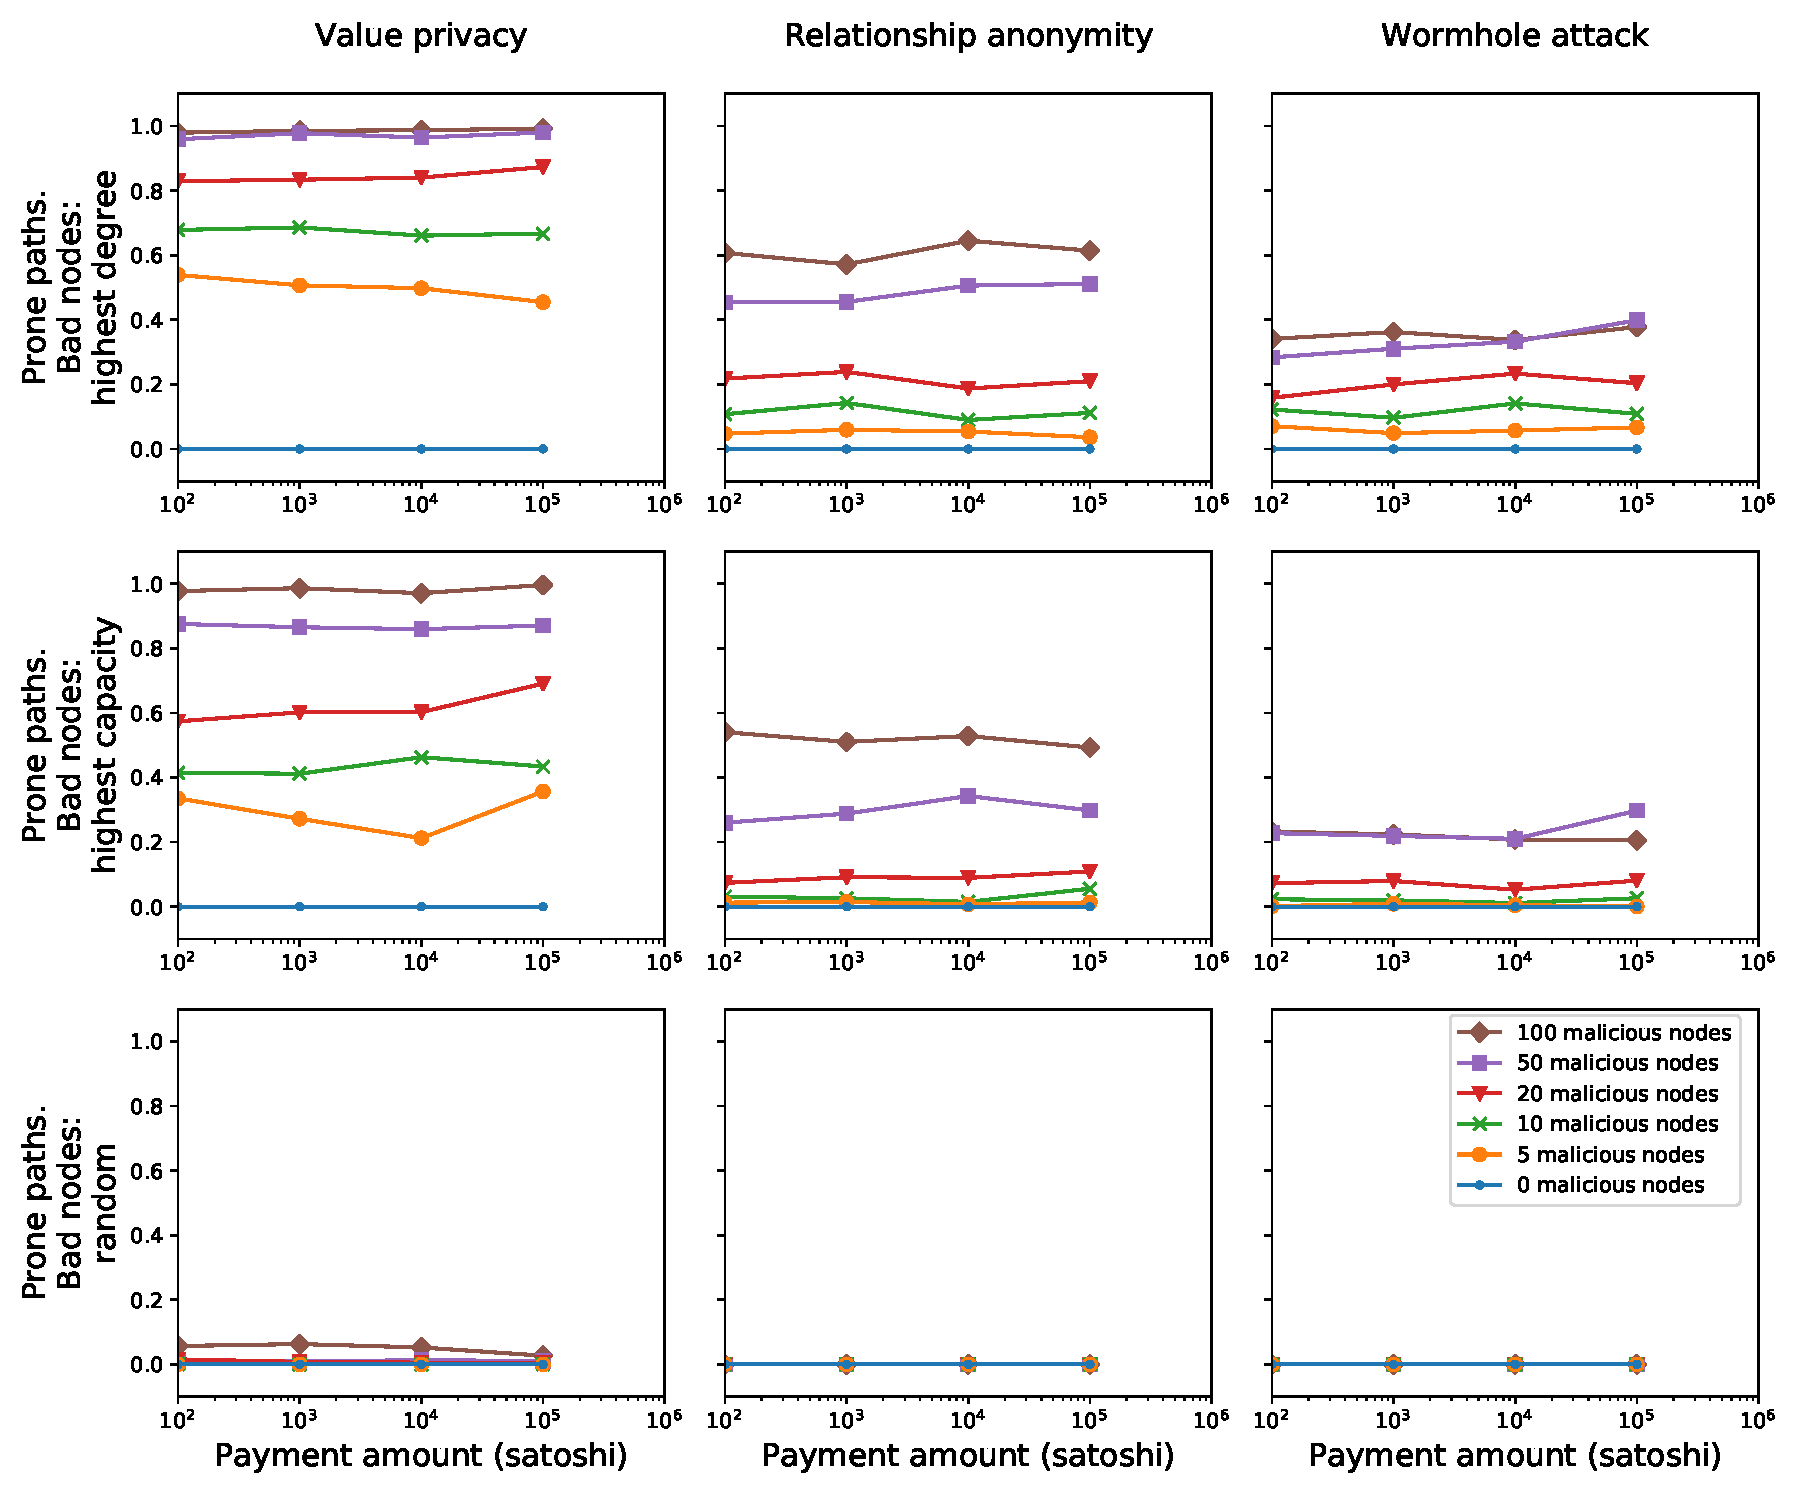
\includegraphics[width=\textwidth]{fig-all-attacks}
	\caption{Share of vulnerable paths for each attack, considering that highest degree nodes are compromised (top), highest capacity nodes are compromised (middle), or random nodes are compromised (bottom).}
	\label{fig:fig-all-attacks}
\end{figure*}

For every attack and a given number of compromised nodes, the share of prone paths is relatively stable for all payment amounts.
This indicates that the payment amount does not significantly affect the security of payments.
% (though it affects the probability of its success as shown in~\cref{fig:payment-success}).

The three attacks differ in how quickly the share of prone paths changes as the number of compromised nodes increases.
For value privacy, the effect of additional highly-connected nodes being compromised is the most profound: 
the share of prone paths is $50\%$ if only the $5$ most connected nodes are compromised 
and nearly $100\%$ if the $100$ most connected nodes are compromised. 
We conclude thus that an adversary needs to corrupt only $2\%$ of the nodes to (almost) completely nullify any value privacy guarantee in the LN.

We observe that the average share of prone paths decreases for relationship anonymity.
Yet, the adversary controlling the $100$ most connected nodes can launch the relationship anonymity attack on about $70\%$ of the paths. 
Interestingly, the adversary has fewer possibilities to launch the wormhole attack.
For instance, even with $100$ most connected nodes corrupted, around $30\%$ of the paths are prone to the attack.
While this is still a crucial security issue, this reduction in the effectiveness of the attack 
may be explained by the fact that the wormhole attack is the most restrictive on path structure, and thus it 
has the lowest share of vulnerable paths. 
%For relationship anonymity, path safety is less sensitive to the increase in the number of compromised nodes: around 90\% and 30\% of paths are safe with 5~and 100~compromised nodes, respectively.

%Finally, the wormhole attack is the least affected, with 90\% and 30\% of safe paths with 5~and 100~compromised nodes.
%This may be explained by the fact that the structure of paths prone to value privacy attack is simpler (one malicious node must be at any point in the path), therefore there are more prone paths.
%Relationship anonymity requires a more elaborate structure (the first and the last nodes are malicious), and there are fewer such paths.
%Finally, wormhole attack is the most restrictive on path structure, and has the lowest share of vulnerable paths.
Increasing the number of compromised nodes results in fewer vulnerable paths if compromised nodes are those with the channels holding the highest capacity, as opposed to highest degree nodes.
This distinction is most profound for relationship anonymity, e.g.,~there are around $50\%$~for $50$~highest degree corrupted nodes, but only around $25\%$~vulnerable paths for $50$~highest capacity corrupted nodes.
%For a roting node to attract payments, good connectivity is more important than high capacity.
This may be explained by the fact that routing algorithms optimize for low path length.
Note that capacity of forwarding channels is not as important as good connectivity, especially for payments of small and medium amounts.

Finally, we consider random nodes compromised instead of the most connected nodes.
%This experiment acts as a baseline for the attack efficiency in the case when the adversary does not have the means to take over professionally maintained nodes.
In contrast to the previous results, we observe that less than $10\%$ of paths are prone to value privacy and nearly no path is prone 
to relationship anonymity and wormhole attack.
We conjecture that this is because randomly selected nodes have few connections (note the degree distribution in Figure~\ref{fig:node-degree-histogram}), and thus their compromise does not affect routing at large.
%Therefore, it is beneficial for an adversary to target highly connected nodes, as this substantially increases the impact of the attack.

%\todo[inline]{@Sergey: Let's have only one path length. It is confusing and hard to parse otherwise.}
%We also perform the same experiments considering longer paths of up to 4 intermediary nodes.
%Due to high computational requirements of the path finding function, we only perform the experiments for 2~amounts (1000 and 100000~satoshis), and 8~iterations.
%The experiments indicate that the increase in the path length by one hop does not significantly affect the results outlined above.

In summary, 
the results of this experiment show that highly connected nodes and nodes with high capacity links have a high impact on the security and privacy of the LN.
Assuming that paths are selected uniformly at random from the set of available paths, 
an adversary that selectively corrupts $100$ (i.e.,~only $2\%$) 
of LN nodes can effectively learn all the transaction values, 
the sender and the receiver for the vast majority of transactions, 
as well as carry out the wormhole attack in about $30\%$ of the paths. 
This shows that the security and privacy attacks shown in theory are indeed crucial in practice. 

Carrying out such an attack might not be infeasible in the live network. We 
note that a large number of highly connected LN nodes is controlled by an unknown entity under the pseudonym LNBIG.
It controls 23~out of top~50 highest connected nodes~\cite{1MLTopConnected} and $40\%$ of the network capacity~\cite{TheBlockLNBIG}.
%This means that a large-scale privacy attack on LN may be performed by compromising LNBIG alone.
%The attacks can further be amplified by using part of LNBIG's capacity to temporarily block other hubs and force more payments to be routed through the compromised nodes.

\subsection{Countermeasures}
We assume in our study that every two nodes carry out their transactions  
along a subset of paths chosen uniformly at random from the set of all available paths between them. 
However, LN nodes might implement different routing strategies. 
%In particular, nodes joining the LN should carefully choose their channel counterparties. 
For instance, while routing through well-connected nodes improves the chances to reach the receiver through a short, highly liquid path, 
the sender might connect to low degree nodes.
This would make the node degree distribution more even at the cost of connectivity and reduce the probability of choosing paths prone to the 
attacks studied in this experiment. 
We envision thus that there is a tradeoff between connectivity on the one hand and security and privacy on the other,
which constitutes a venue for future work.
A node may also route transactions through a trusted proxy node, 
thus guaranteeing that the first node in a path is not compromised.
This would mitigate the relationship anonymity and wormhole attacks (if the total path length is bounded to contain at most three intermediaries).
As the LN protocol is still evolving, the results of the experiments presented in this section should be considered 
for the next design decisions.

Routing protocols for the LN is an active research area~\cite{Roos2018, Sivaraman2018, Malavolta2017a, Prihodko2016, Grunspan2018, Bagaria2019, Osuntokun2018, Pickhardt2019, ZmnSCPxj2019, ZmnSCPxj2019a, ZmnSCPxj2019b}.
The results of our experiments suggest that, although largely omitted so far, 
the security and privacy attacks here studied are a crucial variable to consider when designing routing protocols. 


\section{Related work}

%We can roughly divide the related literature in two groups: academic analyses of the concept of payment-channel networks (PCN)
%and experimental analyses of the Lightning Network data.

Multiple research works have shed light on various aspects of payment-channel networks, such as security~\cite{Malavolta2019, Kiayias2019}, privacy~\cite{Malavolta2017, HerreraJoancomarti2019}, concurrency~\cite{Malavolta2017}, routing~\cite{Malavolta2017a, Roos2018, Sivaraman2018, Prihodko2016}, liquidity~\cite{Dandekar2011,MorenoSanchez2018}, efficiency~\cite{Decker2018}, and incentive compatibility~\cite{Engelmann2017}.
These works mainly share the lack of a quantitative analysis of the impact of their findings in the current LN.
%In tour work , we have empirically analyzed the potential severity of the wormhole attack, 
%as well as attacks on value privacy and relationship anonymity, in the current Lightning Network. 

A group of papers more closely related to ours conveys experimental analyses of various aspects of the LN.
Herrera-Joancomart\'{i} et al.~\cite{HerreraJoancomarti2019} describe an adversarial 
strategy to determine the current balance of a channel in the network.
Tang et al.~\cite{Tang2019} study 
the tradeoffs between balance privacy and routing effectiveness. 
Martinazzi~\cite{Martinazzi2019} and Seres et al.~\cite{Seres2019} study the evolution of topological aspects of the LN graph.
Conoscenti et al.~\cite{Conoscenti2019} study the dependency of the LN on payment hubs 
and the rebalancing mechanisms that ameliorate the effect of depleted channels.

%their estimated cost of attacking one node is $15$~EUR ($16.5$~USD), whereas the cost of attacking the whole LN in our case is estimated at $3000$~USD, i.e.,~around $0.6$~USD per node.


\section{Conclusion}
\label{sec:conclusions}

The Lightning Network (LN) has emerged as the most widely deployed solution for the scalability issue affecting current blockchains such as Bitcoin. 
%Its substantial growth in the number of nodes, payment channels and their capacity has attracted attention from academia and industry.
Despite its conceptual appeal and growing adoption,  several works~\cite{Malavolta2017, Malavolta2019} have identified 
 security, anonymity and scalability limitations. A quantitative 
analysis of their impact, however, is missing and this paper aims at filling this gap.

We quantitatively study for the first time the proneness of the current Lightning Network to the 
wormhole attack as well as attacks against value privacy and relationship anonymity. 
We observe that a moderately resourceful adversary controlling only $2\%$ of the total node count can carry out these attacks with high success probability.

%First, we quantitatively analyze the effect of the wormhole attack as well as attacks on value privacy and relationship anonymity. 
%Second, we quantitatively analyze the restriction of the LN scalability gain due to the limited concurrency supported by the LN protocol. 
%In particular, we observe that more than up to $50\%$ of LN channels can support fewer concurrent micropayments than in principle allowed by their capacity. 
%For instance, the adversary investing $225$k~USD can prevent nodes in the largest community from transacting with the rest of the network. 

% the probability of three privacy attacks depending on payment amounts and the number of compromised nodes.
%Our results show that a payment's probability of being forwarded through a malicious path does not depend on its size, but large payments are less likely to succeed at all.
%Among the three attacks we considered, value privacy is the most sensitive to the number of compromised nodes.
%With just a few highly-connected hubs compromised, LN users risk having their payment amounts leaked to the adversary.
%Relationship anonymity attack and, finally, the wormhole attack are less likely with the same number of malicious nodes.

%Then, we have described an understudied drawback of LN -- the limit on the number of concurrent in-flight payments (HTLCs) in a channel.
%This limitation is explained by the interaction between Lightning and Bitcoin protocols.
%We have shown, first, that this is the key factor limiting LN performance for small payments.
%Our results indicate that some of the widely discussed LN use cases (such as micropayments) might not be viable even with sufficient channel capacity.
%We describe a DoS attack vector based on the HTLC limit and show that it is more efficient for the attacker to block channels by depleting their HTLC limit rather than capacity, as has been already described in the literature.
%In this state of affairs, we prompt the LN community to implement countermeasures to alleviate these security, anonymity and scalability issues. 
%For instance,  we argue that implementing anonymous multi-hop locks (AMHL) instead of the currently used HTLC construction would 
%mitigate the security, privacy  and scalability issues.  %We hope that this work helps Lightning and Bitcoin communities identify and address the most pressing bottlenecks of these technologies and help them achieve their full potential.

